\documentclass[10pt]{article}
\usepackage{fullpage}
\usepackage{url}
\usepackage{color}
\usepackage{listings}

\definecolor{dkgreen}{rgb}{0,0.6,0}
\definecolor{dkred}{rgb}{0.6,0,0}
\definecolor{dkblue}{rgb}{0,0,0.7}

\usepackage{tikz}
\usetikzlibrary{automata, positioning, arrows}
\tikzset{%
  node distance=2.5cm,  
  initial text={},      
  every state/.style={  
    semithick},
  double distance=2pt,  % Accept state appearance
  every edge/.style={   
    draw,
    ->,
    >=stealth',
    auto,
    semithick} %
}

\lstdefinestyle{jvm}{
  % aboveskip=3mm,
  % belowskip=3mm,
  xleftmargin=2em,
  % xrightmargin=2em,
  showstringspaces=false,
  columns=flexible,
  basicstyle={\ttfamily},
  numbers=left,
  moredelim=[s][\color{black}]{Ljava}{;},
  morecomment=[l][\color{dkgreen}]{;},
  morecomment=[l][\color{magenta}]{;;},
  keywords={class,public,static,super,method,code,end},
  keywordstyle=\color{dkblue},
  breaklines=true,
  breakatwhitespace=true,
  tabsize=8
}

\renewcommand{\thepage}{~}

\title{COM S 440/540 Homework 8}
\date{}
\author{Basic blocks and flow graphs}

\begin{document}

\maketitle

\noindent
Reminder: present your own work and properly cite any sources used.
Solutions should be written satisfying the \emph{other student viewpoint},
and must be prepared using \LaTeX.
\renewcommand{\thepage}{~}
%============================================================
\section*{Question~1~\hfill 20 points}
%============================================================
Determine the basic blocks for the following Java assembly code.
\begin{lstlisting}[style=jvm,numbers=none]
.method public static primes : (I)V
    .code stack 4 locals 4
        L03:  iconst_2
        L04:  invokestatic Method primes print (I)V
        L05:  iconst_3
        L06:  istore_1
        L07:  goto L38
        L08:  iconst_1
        L09:  istore_3
        L10:  iconst_3
        L11:  istore_2
        L12:  goto L25
        L13:  iconst_0
        L14:  iload_1
        L15:  iload_2
        L16:  irem
        L17:  if_icmpne L21
        L18:  iconst_0
        L19:  istore_3
        L20:  goto L30
        L21:  iload_2
        L22:  iconst_2
        L23:  iadd
        L24:  istore_2
        L25:  iload_2
        L26:  iload_2
        L27:  imul
        L28:  iload_1
        L29:  if_icmple L13
        L30:  iload_3
        L31:  ifeq L34
        L32:  iload_1
        L33:  invokestatic Method primes print (I)V
        L34:  iload_1
        L35:  iconst_2
        L36:  iadd
        L37:  istore_1
        L38:  iload_1
        L39:  iload_0
        L40:  if_icmple L08
        L41:  return
    .end code
.end method
\end{lstlisting}


%============================================================
\section*{Question~2~\hfill 20 points}
%============================================================

\begin{center}
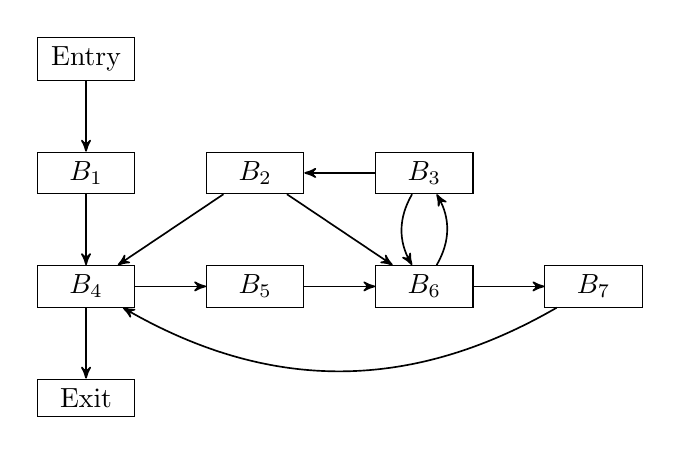
\begin{tikzpicture}
    \matrix[nodes={draw, rectangle, text width=1cm, align=center},
      row sep=9mm, column sep=9mm] {
        \node (B0) {Entry}; \\
        \node (B1) {$B_1$}; & \node (B2) {$B_2$}; & \node (B3) {$B_3$};\\
        \node (B4) {$B_4$}; & \node (B5) {$B_5$}; &
        \node (B6) {$B_6$}; & \node (B7) {$B_7$}; \\
        \node (BN) {Exit}; \\
    };

    \draw
      (B0) edge (B1)
      (B1) edge (B4)
      (B4) edge (BN)
      (B4) edge (B5)
      (B5) edge (B6)
      (B6) edge (B7)
      (B6) edge [bend right] (B3)
      (B3) edge [bend right] (B6)
      (B3) edge (B2)
      (B2) edge (B4)
      (B2) edge (B6)
      (B7) edge [bend left] (B4)
    ;

\end{tikzpicture}
\end{center}
For the flow graph shown above,
identify the loops.
For each loop, give the loop entry.

\end{document}
